\normalsize This section reports changes in mortality from 1992--1994 to 2016--2018 calculated under different assumptions and parameters. We focus on the sensitivity of estimates in Figure \ref{fig:mort_main} for non-Hispanic white women; results for other groups are similarly robust to the specifications here.

\textbf{Percentile Bins Defined in 1992.}  The main figure was calculated using education percentile bins from approximately the middle of the sample in 2003. In that year dropouts accounted for percentiles 0--10, high school graduates for percentiles 10--45, individuals with some college for percentiles 45--70, and individuals with a B.A. or higher accounted for the top 30\%. In 1992, these four education levels respectively represented percentiles 0--17, 17--60, 60--81 and 81--100. Panel A of Figure \ref{fig:robust} shows estimates of mortality change from 1992--94 to 2016--2018 using the latter bin boundaries. The broad patterns of mortality change are the same. Mortality changes are slightly smaller in the bottom group, but this is what we would expect given that the bottom group is now defined as the bottom 17\% rather than the bottom 10\%. The overall divergence of mortality by education is unambiguous.

\vspace{6mm} \textbf{Ranking within Race and Gender.} The body of the paper ranks individuals against members of their own gender. It thus reports, for example, changes in mortality for white women in the bottom 10\% of the female education distribution. An alternate approach is to define percentiles within race and gender, and thus to examine mortality changes for white women in the bottom 10\% of the white women's education distribution. This approach would be sensible if one's relative position in the own-race socioeconomic distribution was an important factor for mortality. Panel B of Figure~\ref{fig:robust} presents the main estimates, where education percentiles are defined within race and gender. The pattern of dramatically rising mortality for whites in the bottom 10\% remains evident. The total increases in mortality are slightly less under this definition, because white education has increased more than black education over this period, but the change in selection bias is small.

\vspace{6mm} \textbf{Alternate Bounding Assumptions.} The main analysis calculated bounds under the assumptions that (i) expected mortality is weakly monotonically declining in latent educational rank for all groups; and (ii) there is an upper bound on the size of kinks or discrete jumps in the expected mortality function.
While these assumptions are sensible and consistent with other
research and data on the expectation of mortality as a function of
education, we can readily relax these assumptions. Although our main
estimates are necessarily less precise under more general assumptions,
none any of the substantive conclusions change. 

Appendix~\ref{sec:app_nonmon} above presents bounds on mortality change as we gradually loosen the monotonicity assumption, and allow mortality to rise with education.

Panel C of Figure~\ref{fig:robust} presents results when we allow the
mortality function to have discrete jumps or kinks of any size when
crossing educational boundaries, for example, when crossing the
threshold of high school completion. Thus Panel C addresses concerns
about sheepskin effects by permitting (but not imposing) mortality to
fall discontinuously at the margin of completing a given education
level. 

Panel D removes the curvature restriction entirely; in this specification, the CEF can have discrete kinks or jumps at any point in the education rank distribution, though it must remain monotonic. In both cases, the key result of substantial mortality gain among the least educated is robust. The other findings of the paper---education divergence among black men and women, and the patterns of deaths of despair---are similarly robust to these specifications.

%%%%%%%%%%%%%%%%%%%%%%%%%%%%%%%%%%%%%%%%%%%%%%
% Figure: Causes of Death -- 1992 Boundaries %
%%%%%%%%%%%%%%%%%%%%%%%%%%%%%%%%%%%%%%%%%%%%%%
\begin{figure}[H]
  \caption{Change in non-Hispanic White Female Mortality: Sensitivity Analysis} \thispagestyle{empty}
  \label{fig:robust}

  \begin{center}
    \vspace{-.6cm} Panel A: 1992 Percentile Boundaries
  \end{center}
  \vspace{-1.4cm}
  \begin{center}
    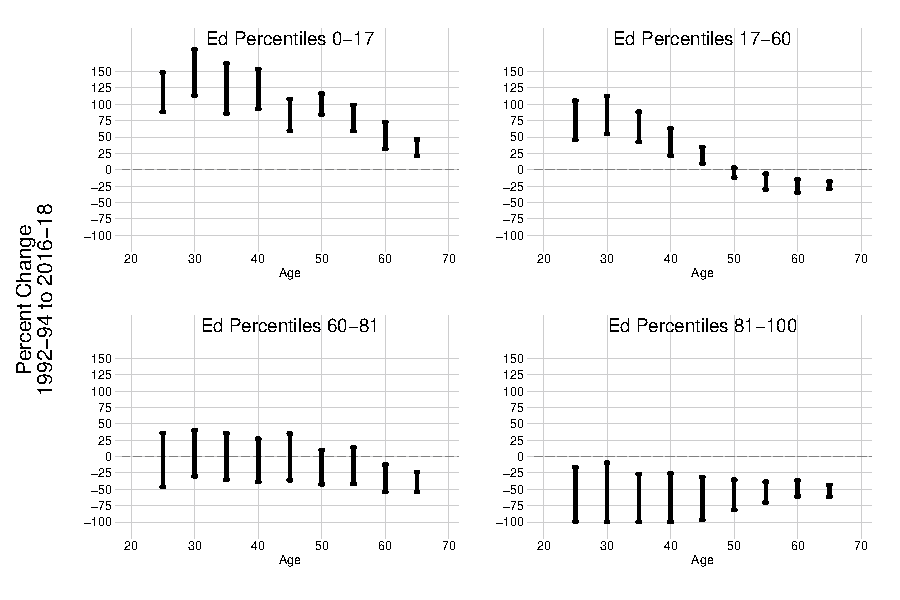
\includegraphics[scale=1.1]{\mortalitypath/causes-1992-2-1} &
  \end{center}

  \begin{center}
    \vspace{-.6cm} Panel B: Within Race-Gender Percentiles
  \end{center}
  \vspace{-1.4cm}
  \begin{center}
    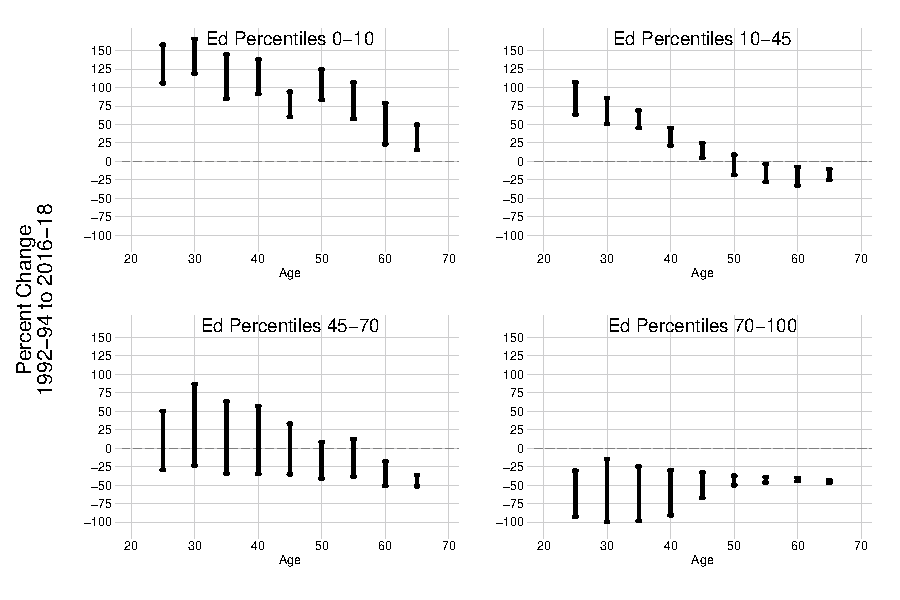
\includegraphics[scale=1.1]{\mortalitypath/causes-racesex-2-1} \\
  \end{center}
\end{figure}

\begin{figure}[H]\ContinuedFloat
  \caption{Change in non-Hispanic White Female Mortality: Sensitivity Analysis (Continued)} \thispagestyle{empty}
  \begin{center}
    \vspace{-.6cm} Panel C: Allow Sheepskin Effects
  \end{center}
  %\vspace{-1.4cm}
  \begin{center}
    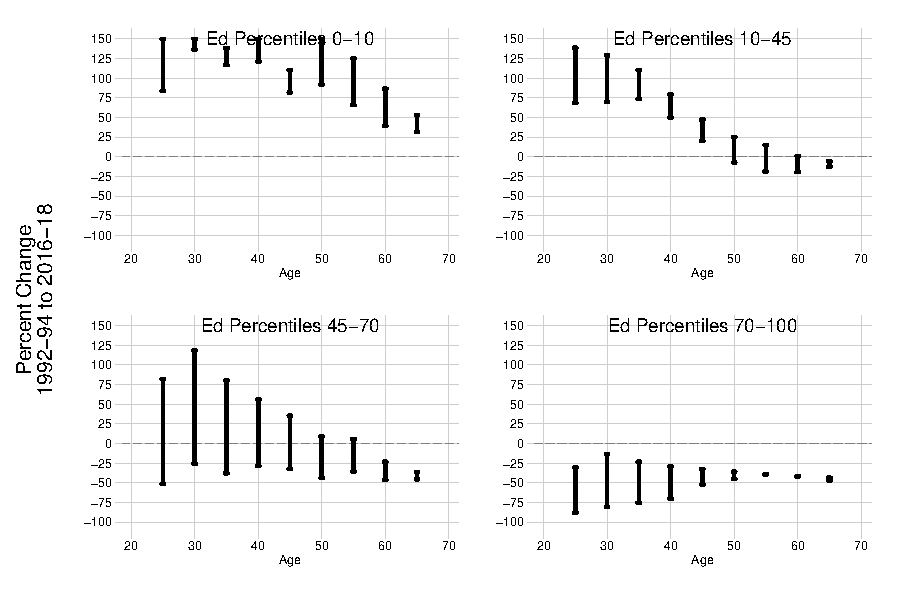
\includegraphics[scale=0.78]{\mortalitypath/causes-mon-step-2-1} \\
  \end{center}

  \begin{center}
    \vspace{-.6cm} Panel D: No Curvature Constraint
  \end{center}
  %\vspace{-1.4cm}
  \begin{center}
    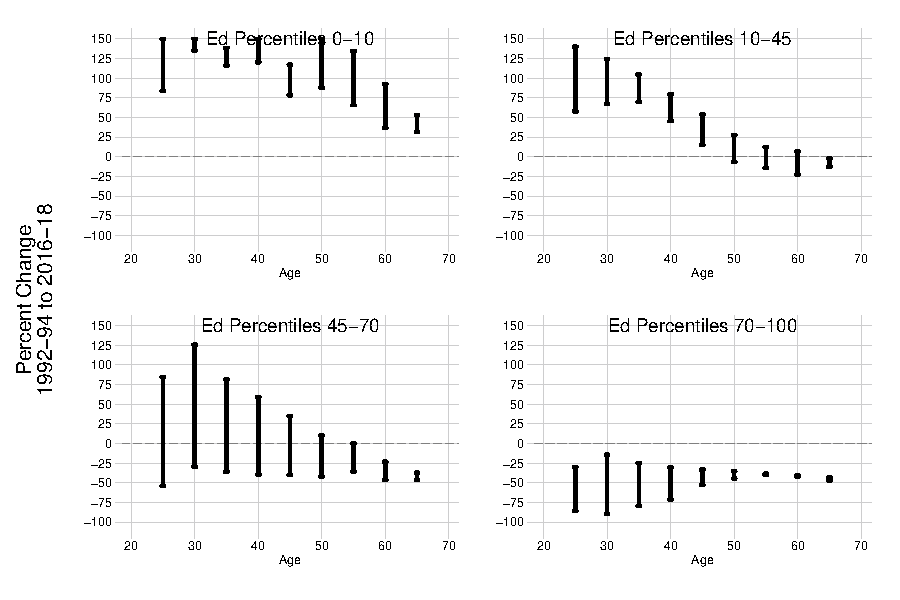
\includegraphics[scale=0.78]{\mortalitypath/causes-nof2-2-1} \\
  \end{center}
\end{figure}
\vspace{-1cm} \tiny{Note: The figure shows bounds on mortality change from 1992--1994 to 2016--2018, for non-Hispanic white women, by age and percentile education bin, under alternate assumptions from the main body of the paper. The figure is analogous to Panel A of Figure~\ref{fig:mort_main}, but with different bounding assumptions. Panel A defines education bins boundaries according to education levels in 1992--1994. Panel B defines an individual's education percentile according to the individual's rank in the own-race and own-gender education distribution, rather than in the own-gender education distribution. Panel C allows sheepskin effects, by allowing kinks and discrete jumps at education boundaries (e.g. the rank separating dropouts from high school completers). Panel D estimates bounds on mortality without restricting the curvature of the mortality-education CEF. The lines show the bounded set containing the percentage change in the mortality rate from 1992--1994 to 2016--2018 for the given group.}

